\documentclass[11pt,a4paper]{article}


\usepackage[utf8]{inputenc}
%\usepackage[latin1]{inputenc}
\usepackage[ngerman]{babel}
\usepackage[T1]{fontenc}
\usepackage{float}
\usepackage{amssymb}
\usepackage{amsmath}
\usepackage{amstext}
\usepackage{listings}
\usepackage{makeidx}
\usepackage{fancyhdr}
\pagestyle{fancyplain}

\usepackage{booktabs} %for top, middle and bottomline
%---
%\usepackage{here} 
% \usepackage{subfigure}
% \usepackage{esvect}
% \usepackage[europeanresistor]{circuitikz}
% \usepackage{tikz}
%-----
\usepackage{capt-of}
%----
% \usepackage{epstopdf}%--enable-write18 oder --shell-escape muss aktiviert sein
%\epstopdfsetup{outdir=./4/}
%----
\pagestyle{fancy}
\usepackage[pdftex]{graphicx}
\usepackage[colorlinks = false]{hyperref}
\usepackage{geometry}
\usepackage{uniinput}
% \usepackage{longtable}
% \usepackage{units}
\usepackage{siunitx}

\geometry{a4paper, top=25mm, left=40mm, right=25mm, bottom=30mm,
headsep=10mm, footskip=12mm}


\newsavebox{\ParaBox}

\newcommand{\Abb}[1]{Abbildung \ref{fig:#1}}
\newcommand{\Abs}[1]{Abschnitt \ref{sec:#1}}
\newcommand{\Gl}[1]{Gleichung \ref{eq:#1}}
\newcommand{\Tab}[1]{Tabelle \ref{tab:#1}}
\newcommand{\EqualO}[1]{\stackrel{(\ref{#1})}{=}}
\newcommand{\EqualT}[2]{\stackrel{(\ref{#1},\ref{#2})}{=}}
\newcommand{\minibild}{7cm}
% \newcommand{•}{\item}

\newcommand{\Ann}[1][/]{\sbox{\ParaBox}{\emph{\textsl{#1}}}\begin{flushright}\usebox{\ParaBox}\end{flushright}}

\numberwithin{equation}{section} 
\renewcommand{\theequation}{\arabic{section}.\arabic{equation}}

\newcommand{\myKapitel}{}
\newcommand{\myUnterkapitel}{}
\renewcommand{\sectionmark}[1]{\renewcommand{\myKapitel}{#1}
\renewcommand{\myUnterkapitel}{}}

\renewcommand{\subsectionmark}[1]{\renewcommand{\myUnterkapitel}{#1}}


\lhead {\begin{minipage}{\minibild } \myKapitel\vspace{1mm}\end{minipage}}%\\ \thepage / \pageref{bla}}
\chead {}

\rhead {\begin{minipage}{\minibild } \flushright\myUnterkapitel\end{minipage}}
\cfoot {}
\rfoot {}

\makeindex

% \renewcommand{\thepage}{\roman{page}}

\newcommand{\initContent}{
    \setcounter{page}{1}
    \renewcommand{\thepage}{\arabic{page}}
}

\newcommand{\initAnhang}{
    \setcounter{page}{1}
    \renewcommand{\thepage}{\Roman{page}}
}

\title{Report of the random ballistic deposition program}

\begin{document}

\lfoot{Heinrich Schmidt}
\maketitle
\tableofcontents

\section{Description of the Random Ballistic Deposition model}
	Random ballistic deposition means, that we generate random x und y coordinates and drop the sphere on this position into a cuboid. The sphere sticks immediatly on the first contact in z-direction with another sphere.
\section{Algorithm}
	The used algorithm splits the cuboid into many subcuboids which stores every sphere which overlapp with the subcuboid. Then all Spheres in the subcubic are sorted by the z-value. If we drop a new sphere we can calculate the minimum possible distance for the new shpere and the upper spheres in the subcuboid until this distance is lower than the twice of the radius.\\
	In case of Polydisperse spheres we must calculate the distance for more than one sphere, because the first z-value of the touching point is relevant and the order of spheres in the subcuboid differs from the order of touchingpounts.
	\begin{figure}
		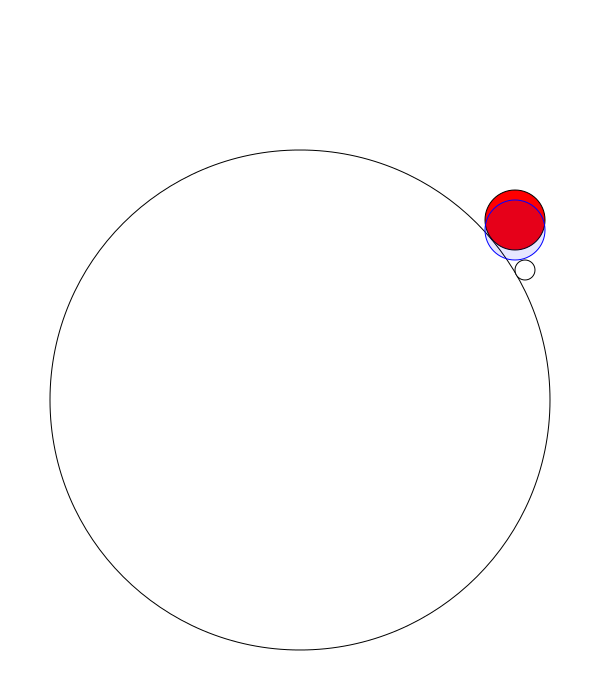
\includegraphics[width=9cm]{figures/polydisperse}
		\caption{the red shpere was added at least. if we use only the first touching sphere when all spheres are sorted by the z-cordinate it would overlapp with the big sphere. for example, the blue sphere do.}
	\end{figure}

\end{document}
